\documentclass[border=10pt]{standalone}
\usepackage{pgfplots}
\usepgfplotslibrary{colormaps}
\pgfplotsset{compat=1.18}

\begin{document}
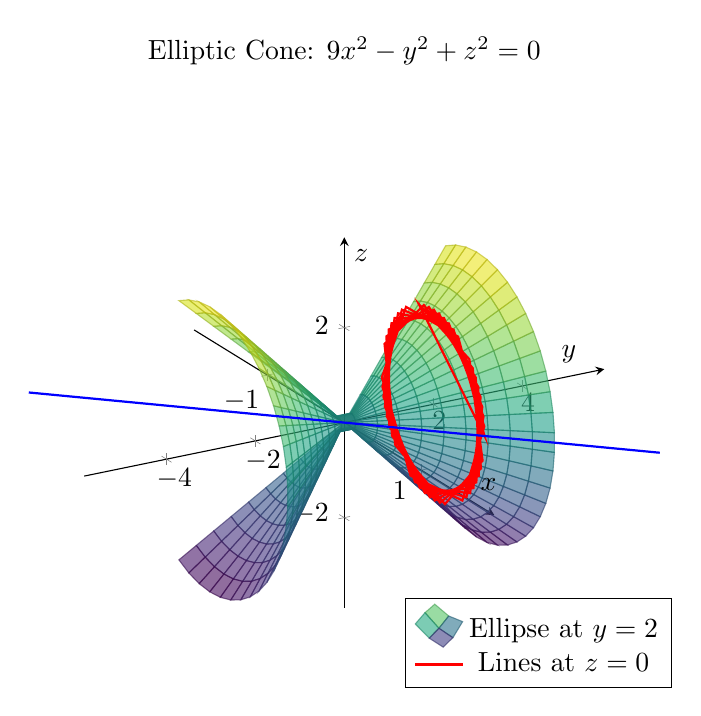
\begin{tikzpicture}
\begin{axis}[
    view={60}{30},
    xlabel={$x$},
    ylabel={$y$},
    zlabel={$z$},
    title={Elliptic Cone: $9x^2 - y^2 + z^2 = 0$},
    width=12cm,
    height=10cm,
    domain=-2:2,
    y domain=-3:3,
    samples=30,
    samples y=20,
    colormap/viridis,
    axis lines=center,
    enlargelimits=0.15,
    grid=major,
    legend style={at={(0.9,0.1)},anchor=south east},
]

% The elliptic cone surface
\addplot3[surf, opacity=0.6] ({abs(y)/3*cos(deg(x))}, {y}, {abs(y)*sin(deg(x))});

% Trace at y = 2 (ellipse)
\addplot3[domain=0:360, samples=50, thick, red] 
    ({2/3*cos(deg(x))}, {2}, {2*sin(deg(x))});
\addlegendentry{Ellipse at $y=2$}

% Trace lines at z = 0
\addplot3[domain=-1.5:1.5, samples=20, thick, blue] (x, {3*x}, 0);
\addlegendentry{Lines at $z=0$}

\end{axis}
\end{tikzpicture}
\end{document}
